\documentclass{article}
\usepackage[utf8]{inputenc}
\usepackage[top=0.1in, left=1.0in, right=1.0in]{geometry}
\usepackage{graphicx}
\usepackage[export]{adjustbox}
\usepackage{latexsym}
\usepackage{amsmath}
\usepackage{amssymb}
\usepackage{tikz}
\usetikzlibrary{calc,shapes.multipart,chains,arrows}
\usepackage{geometry,mathtools}
\setcounter{MaxMatrixCols}{19}
\usepackage[russian]{babel}
\usepackage[T2A]{fontenc}
\usepackage{amsfonts}
\usepackage{graphicx}
\title{ \textbf{Дискретная Mатематика} }
\author{\textbf{ФИО : Анужин Баатарцогт \ \ M3112}  }
\date{25 March 2020}
\begin{document}
\maketitle
\vspace{-0.15in}
	\vspace{0.05in}
	
\section{\Large{(2 балла)Для двух данных функций сделать одну подстановку и одно отождествление}}
\Large{\textbf{$f(x, y) = \overline{x} \nrightarrow \overline{y+x}$
$f(x, y) = \overline{x} \nrightarrow \overline{y+x}$
$= \overline{x}({y+x}) $
$= \overline{x}{y} $
}}

\bigskip

\textbf{$g(a , b , c, d) = a \downarrow b \nleftarrow {c \mid d} $
$= \overline{a} \ \overline{b} \nleftarrow{\overline{c} + \overline{d}}$
$= \overline{\overline{a}  \overline{b}}(\overline{c} + \overline{d})$
$= (a+b)(\overline{c} \ + \overline{d})$}

\subsection*{}
\textbf{Подстановка:}

$h(x, g(a,b,c,d))= \overline{x}(a+b)(\overline{c} \ + \overline{d})$
\bigskip

\textbf{Отождествление:}

$g(a , b , c, d) = {(a+b)}(\overline{c} \ + \overline{d})$

$h(a, b, c, a) = {(a+b)}(\overline {c} + \overline {a})$

$=  {a}\overline{c} + b\overline{c} + \overline{a}{b}$

\section{\Large{(2 балла) Запишите для графа:\newline\\1. матрицу смежности;\\
2. инцидентности;\\
3. список смежности;\\
4. степени вершин.}} \\ \newline \newline
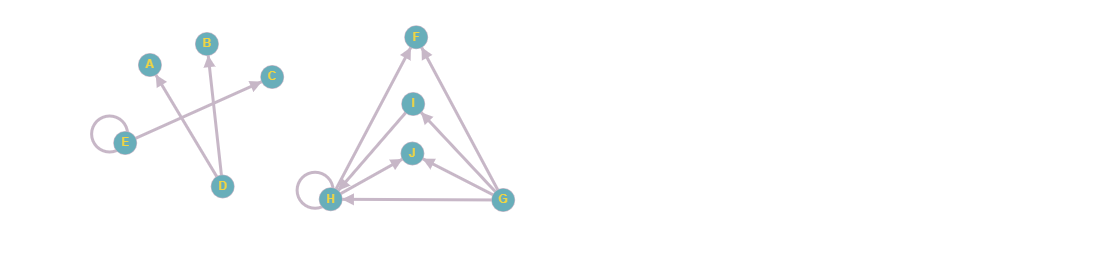
\includegraphics[width=\textwidth,height=\textheight,keepaspectratio]{2.1.png}

\Large{\textbf{1. матрицу смежности;}}

\[
\begin{matrix*}[r]
  & a & b & c & d & e & f & g & h & i & j\\
a & 0 & 0 & 0 & 0 & 0 & 0 & 0 & 0 & 0 & 0\\
b & 0 & 0 & 0 & 0 & 0 & 0 & 0 & 0 & 0 & 0\\
c & 0 & 0 & 0 & 0 & 0 & 0 & 0 & 0 & 0 & 0\\
d & 1 & 1 & 0 & 0 & 0 & 0 & 0 & 0 & 0 & 0\\
e & 0 & 0 & 1 & 0 & 1 & 0 & 0 & 0 & 0 & 0\\
f & 0 & 0 & 0 & 0 & 0 & 0 & 0 & 0 & 0 & 0\\
g & 0 & 0 & 0 & 0 & 0 & 1 & 0 & 1 & 1 & 1\\
h & 0 & 0 & 0 & 0 & 0 & 1 & 0 & 1 & 0 & 1\\
i & 0 & 0 & 0 & 0 & 0 & 0 & 0 & 1 & 0 & 0\\
j & 0 & 0 & 0 & 0 & 0 & 0 & 0 & 0 & 0 & 0\\
\end{matrix*} 
\]
\newline
\Large{\textbf{2. инцидентности;}}\\
\[
\begin{matrix*}[r]
   & da & db & ec & ee & gf & gi & gj & gh & ih & jh & hf & hh\\
a &  1 &  0 &  0 &  0 &  0 &  0 &  0 &  0 &  0 &  0 &  0 &  0\\
b &  0 &  1 &  0 &  0 &  0 &  0 &  0 &  0 &  0 &  0 &  0 &  0\\
c &  0 &  0 &  1 &  0 &  0 &  0 &  0 &  0 &  0 &  0 &  0 &  0\\
d & -1 & -1 &  0 &  0 &  0 &  0 &  0 &  0 &  0 &  0 &  0 &  0\\
e &  0 &  0 & -1 &  2 &  0 &  0 &  0 &  0 &  0 &  0 &  0 &  0\\
f &  0 &  0 &  0 &  0 &  1 &  0 &  0 &  0 &  0 &  0 &  1 &  0\\
g &  0 &  0 &  0 &  0 & -1 & -1 & -1 & -1 &  0 &  0 &  0 &  0\\
h &  0 &  0 &  0 &  0 &  0 &  0 &  0 &  1 &  1 &  1 & -1 &  2\\
i &  0 &  0 &  0 &  0 &  0 &  1 &  0 &  0 & -1 &  0 &  0 &  0\\
j &  0 &  0 &  0 &  0 &  0 &  0 &  1 &  0 &  0 & -1 &  0 &  0\\
\end{matrix*}
\]
\\\\
%\newpage
\Large{\textbf{3. список смежности;}}\\ \\
\Large{\textbf{$a: \  \emptyset$}}\\ \\
\Large{\textbf{$b: \ \emptyset$}}\\ \\
\Large{\textbf{$c: \  \emptyset$}}\\ \\
\Large{\textbf{$d: \ a, b$}}\\ \\
\Large{\textbf{$e: \ e, c $}}\\ \\
\Large{\textbf{$f: \ \emptyset$}}\\ \\
\Large{\textbf{$g: \ f, i, j, h$}}\\ \\
\Large{\textbf{$h: \ j, f, h$}}\\ \\
\Large{\textbf{$i: \ h$}}\\ \\
\Large{\textbf{$j: \ \emptyset$}}\\\\

\Large{\textbf{4. степени вершин}}\\\\
\large\textbf{\textit{InDeg }– число ребра, входящих в данную вершину.}\newline
\large\textbf{\textit{OutDeg}– число ребра, выходящих из данной вершины.}\newline
\\
\Large{\textbf{$InDeg(a) = 0 \hspace{2cm} OutDeg(a) = 1 $}}\\
\Large{\textbf{$InDeg(b) = 0 \hspace{2cm} OutDeg(b) = 1 $}}\\
\Large{\textbf{$InDeg(c) = 0 \hspace{2cm} OutDeg(c) = 1 $}}\\
\Large{\textbf{$InDeg(d) = 2 \hspace{2cm} OutDeg(d) = 0 $}}\\
\Large{\textbf{$InDeg(e) = 2 \hspace{2cm} OutDeg(e) = 1 $}}\\
\Large{\textbf{$InDeg(f) = 0 \hspace{2cm} OutDeg(f) = 2 $}}\\
\Large{\textbf{$InDeg(g) = 4 \hspace{2cm} OutDeg(g) = 0 $}}\\
\Large{\textbf{$InDeg(h) = 3 \hspace{2cm} OutDeg(h) = 3 $}}\\
\Large{\textbf{$InDeg(i) = 1 \hspace{2cm} OutDeg(h) = 1 $}}\\
\Large{\textbf{$InDeg(j) = 0 \hspace{2cm} OutDeg(h) = 2 $}}\\\\

\section{\Large{ (2 балла) Найти для указанного графа и дополнительного к
нему: \\ 1. центр; \\2. диаметр; \\ 3. радиус.
}}

\begin{figure}[h]
    \centering
    
\includegraphics[width=\textwidth,height=\textheight,keepaspectratio]{3.png}
    \caption{Граф}
    \label{fig:my_label}
\end{figure}

\subsection*{Решение:}
\textbf{Эксцентриситетом $\epsilon(v)$} вершины $v$ называется наибольшее геодезическое расстояние между $v$ и любой другой вершиной графа. \\
${\displaystyle \epsilon (v)=\max _{u\in V}d(v,u)}$ 
\bigskip

$\epsilon(a) = 2$

$\epsilon(b) = 3$

$\epsilon(c) = 2$

$\epsilon(d) = 3$

$\epsilon(e) = 2$

$\epsilon(f) = 3$

$\epsilon(g) = 2$

$\epsilon(h) = 3$

\bigskip

\textbf{Радиусом $r$} графа называется минимальный эксцентриситет среди всех вершин графа

${\displaystyle r=\min _{v\in V}\epsilon (v)}$ , 
\Large\textbf{} r(G) = 2

\bigskip

\textbf{Диаметром $d$} графа называется максимальный эксцентриситет среди всех вершин графа. Таким образом, $d$ расстояние между всеми парами вершин графа

${\displaystyle d=\max _{v\in V}\epsilon (v)}$

\bigskip
 d(G) = 3.

\bigskip
\textbf{Центральной вершиной} графа радиусом $r$ называется вершина, на которой достигается радиус.

${\displaystyle \epsilon (v)=r}.$

\bigskip


Итак, центральные вершины.  v =  \{a, c, e, g\}.

\bigskip

\Large\textbf{Теперь мы используем тот же метод с дополнительным графом:}
\bigskip
\begin{figure}[h]
    \centering
    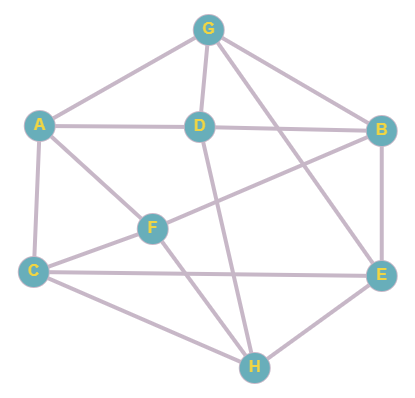
\includegraphics[width=.6\textwidth]{3extra.png}
    \caption{Граф}
    \label{fig:my_label}
\end{figure}

Находим эксцентриситет для всех вершин:

$\epsilon(a) = 2$

$\epsilon(b) = 2$

$\epsilon(c) = 2$

$\epsilon(d) = 2$

$\epsilon(e) = 2$

$\epsilon(f) = 2$

$\epsilon(g) = 2$

$\epsilon(h) = 2$
 \newline
r(G) = 2, d(G) = 2, v = \{a, b, c, d, e, f, g, h\}.

\section{\Large{ (4 балла) Запишите для представленного графа и дополнительного к нему: \\ 1. компоненты реберной двусвязности;
 \\2. компоненты вершинной двусвзяности; \\ 3. точки сочленения, если их нет, то укажите почему; \\ 4. мосты, если их нет, то укажите почему
}}

\begin{figure}[h]
    \centering
    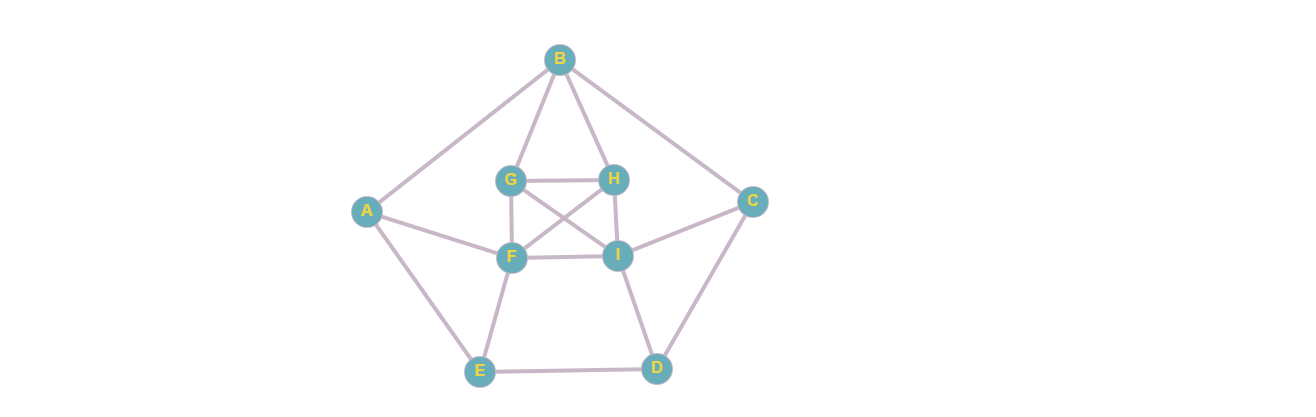
\includegraphics[width=\textwidth,height=\textheight,keepaspectratio]{4.png}
    \caption{Граф}
    \label{fig:my_label}
\end{figure}
\subsection*{Решение:}

\large{\textbf{1. Компоненты реберной двусвязности: Весь Граф. В этом графе сушествует 2  рёберных непересекаюшихся пути.}}\newline \\
\large{\textbf{2. Компоненты вершинной двусвзяности: Весь Граф. В этом графе сушествует 2 вершинных непересекаюшихся пути.}}\newline\\
\large{\textbf{3. Точки сочленения: нет. Одна компонента связности, то есть при удалений вершин, компоненты не увеличивается. }}\newline\\
\large{\textbf{4. Мосты: нет. Одна компонента связности, то есть при удалений ребра, компоненты не увеличивается.}}\newline
\newpage
\Large\textbf{Теперь мы используем тот же метод с дополнительным графом:}
\begin{figure}[h]
    \centering
    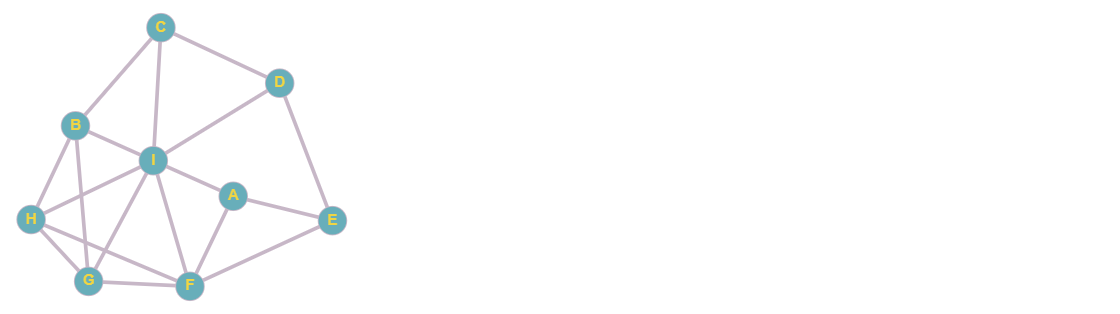
\includegraphics[width=\textwidth,height=\textheight,keepaspectratio]{4 dop.png}
    \caption{Граф}
    \label{fig:my_label}
\end{figure}
\subsection*{Решение:}

\large{\textbf{1. Компоненты реберной двусвязности: Весь Граф. В этом графе сушествует 2  рёберных непересекаюшихся пути.}}\newline \\
\large{\textbf{2. Компоненты вершинной двусвзяности: Весь Граф. В этом графе сушествует 2 вершинных непересекаюшихся пути.}}\newline\\
\large{\textbf{3. Точки сочленения: нет. Одна компонента связности, то есть при удалений вершин, компоненты не увеличивается. }}\newline\\
\large{\textbf{4. Мосты: нет. Одна компонента связности, то есть при удалений ребра, компоненты не увеличивается.}}\newline
\end{document}
